\chapter{Lois de comportement} \label{chap:Ch04}
\section{Problèmes de mécanique des solides} \label{sec:Ch04-1}
\subsection{Formulations dynamiques et quasi-statiques}  \label{ssec:Ch04-1.1}
Pour résoudre un problème de Mécanique des Solides, il faut calculer la solution $(u_i, \sigma_{ij})$, c'est-à-dire calculer les champs de vecteurs déplacements $u_i(x)$ et de tenseurs des contraintes $\sigma_{ij}(x)$, à partir des données, qui sont constituées par
\begin{enumerate}
    \item l'ensemble des sollicitations imposées au solide:
        \begin{itemize}
            \item forces volumiques;
            \item conditions aux limites (forces ou déplacements imposés à la surface).
        \end{itemize}
    \item les conditions initiales, précisant la position et la vitesse initiale du solide.
\end{enumerate}
\textbf{Exemple:} Réservoir sphérique soumis à une pression intérieure $n$
\begin{center}
    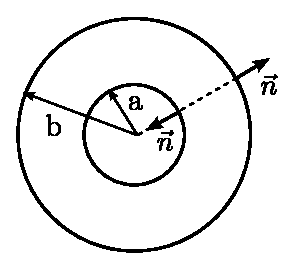
\includegraphics{../images/T1_Ch04-0001}
\end{center}
\begin{itemize}
    \item les forces volumiques sont supposées nulles (pesanteur négligeable)
        \begin{equation}
            f_i = 0
            \label{eq:Ch04-001}
        \end{equation}
    \item la surface extérieure $r=b$ est soumise à la pression atmosphérique, la contrainte est donc nulle d'après~\eqref{eq:Ch02-002}:
        \begin{equation}
            r=b:\quad \sigma_{ij} n_j = T_i = 0
            \label{eq:Ch04-002}
        \end{equation}
    \item la surface intérieure $r=a$ est soumise à la pression $p$ (supposée mesurée par rapport à la pression atmosphérique) d'où
        \begin{equation}
            r=a:\quad \sigma_{ij} n_j = T_i = -p n_i
            \label{eq:Ch04-003}
        \end{equation}
\end{itemize}
\begin{enumerate}
    \item problème dynamique: on  donne  la pression  $p(t)$  comme  fonction  du  temps; on  donne  également les  conditions  initiales  -- par  exemple,  à  $t=0$,  le réservoir est au repos
        \begin{equation}
            u_i(x,0)=0 \quad V_i(x,0) = \frac{\partial u_i}{\partial t}(x,0) = 0
            \label{eq:Ch04-004}
        \end{equation}
        et on cherche la solution $u_i(x,t),\ \sigma_{ij}(x,t)$ qm doit vérifier l'équation du mouvement~\eqref{eq:Ch03-028}
        \begin{equation}
            \rho_0 \frac{\partial^2 u_i}{\partial t^2} = \frac{\partial \sigma_{ij}}{\partial x_j} + f_i
            \label{eq:Ch04-005}
        \end{equation}
        avec~\eqref{eq:Ch04-001}, les conditions aux limites~\eqref{eq:Ch04-002} et~\eqref{eq:Ch04-003}, et les conditions initiales~\eqref{eq:Ch04-004}.
        Ce problème correspond par exemple à l'étude de la mise en charge brutale du réservoir.
        Moyennant une modification des conditions initiales~\eqref{eq:Ch04-004}, il correspond aussi à l'étude des vibrations du réservoir, si l'on impose une pression $p(t)$ sinusoïdale
        \begin{equation}
            p(t) = p_0 \cos \omega t
            \label{eq:Ch04-006}
        \end{equation}
        on recherche alors une solution périodique en $t$, condition qui remplace~\eqref{eq:Ch04-004}.
    \item problème statique: la pression $p$ est constante c'est la pression en service du réservoir.
        On recherche alros une solution statique, c'est-à-dire indépendante du temps $u_i(x),\ \sigma_{ij}(x)$ vérifiant les équations d'équilibre
        \begin{equation}
            \frac{\partial \sigma_{ij}}{\partial x_j} +f_i = 0
            \label{eq:Ch04-007}
        \end{equation}
        avec~\eqref{eq:Ch04-001} et les CI (conditions aux limites)~\eqref{eq:Ch04-002} et~\eqref{eq:Ch04-003}.
        Le temps a disparu, et les conditions initiales n'ont plus lieu d'être.
    \item Problème quasi-statique: On suppose comme en a) que la pression $t$ varie au cours du temps, $p(t)$, mais on fait l'hypothèse quasi-statique: les évolutions sont suffisamment lentes pour que, dans l'équation du mouvement~\eqref{eq:Ch04-005}, on puisse négliger le terme d'accélération et donc la remplacer par l'équation d'équilibre~\eqref{eq:Ch04-007}. En d'autres termes, la sollicitation dépend du temps, mais on résoud à chaque instant un problème statique. Cette hypothèse est tout à fait essentielle en mécanique des solides, car elle permet de ramener à des problèmes statiques les problèmes réels qui, eux, dépendent toujours du temps. L'essentiel de ce cours sera désormais limité au cas où cette hypothèse est valable, l'étude des problèmes réellement dynamiques (chocs, vibrations) étant renvoyée au cours de Mécanique des Vibrations.
\end{enumerate}
\subsection{Conditions aux limites} \label{ssec:Ch04-1.2}
\textbf{Exemple 2.} Ecrasement d'un lopin entre les deux plateaux rigides d'une presse:

\begin{wrapfigure}[12]{l}{6.5cm}
    \begin{center}
        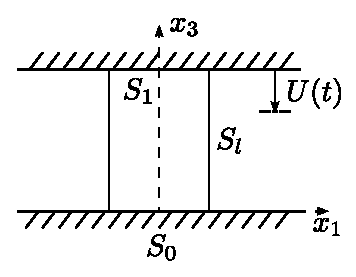
\includegraphics{../images/T1_Ch04-0002}
    \end{center}
\end{wrapfigure}
Un bloc métallique cylindrique est écrasé entre les deux plateaux rigides d'une presse.
Le plateau inférieur $x_3 =0$ est immobile, tandis que le plateau supérieur $x_3 =h$ s'enfonce d'une longueur $U(t)$.
À nouveau, on peut s'intéresser aux problèmes dynamique, statique ou quasi-statique, mais nous nous limiterons au dernier cas: la solution dépend du temps puisque la sollicitation en dépend, mais nous écrirons néanmoins les équations d'équilibre de la statique.

Comme dans l'exemple précédent, et comme dans la majorité des cas en Mécanique des Solides, la seule force de volume est la pesanteur, et nous la négligerons, d'où~\eqref{eq:Ch04-001}.
La surface latérale $S_\ell$ est libre de contraintes
\begin{equation}
    \text{sur } S_\ell:\quad T_i = \sigma_{ij} n_j = 0
    \label{eq:Ch04-008}
\end{equation}
Sur les extrémités $S_0$ $(x_3=0)$ et $S_\ell$ $(x_3=h)$, la condition exprimant la rigidité des plateaux porte sur le déplacement vertical
\begin{equation}
    \begin{aligned}
        & x_3=0:\quad&& u_3 = 0 \\
        & x_3=h: && u_3 = -U(t)
    \end{aligned}
    \label{eq:Ch04-009}
\end{equation}
mais les autres conditions aux limites dépendent des conditions de contact entre les plateaux et le lopin.

\emph{S'il n'y a pas de frottement}, c'est-à-dire si le contact est parfaitement lubrifié, alors la force de contact, qui est donnée par exemple, en $x_3=h$, par
\begin{equation}
    \vec{n} = \left( 0,0,+1 \right), \quad \vec{T} = \left( \sigma_{13}, \sigma_{23}, \sigma_{33} \right)
    \label{eq:Ch04-010}
\end{equation}
doit être normale à la surface de contact.
Les conditions~\eqref{eq:Ch04-009} doivent être complétées par les conditions $\sigma_{13} = \sigma_{23} = 0$
\begin{equation}
    \begin{aligned}
        &x_3 = 0:\quad && u_3 = 0, & \sigma_{13} = \sigma_{23} = 0 \\
        &x_3 = h: && u_3 = -U(t), & \sigma_{13} = \sigma_{23} = 0
    \end{aligned}
    \label{eq:Ch04-011}
\end{equation}
\emph{S'il n'y a pas de glissement}, c'est-à-dire s'il y a adhérence complète entre le lopin et le plateau, alors il faut compléter~\eqref{eq:Ch04-009} par les conditions cinématiques d'adhérence $u_1 = u_2 = 0$
\begin{equation}
    \begin{aligned}
        &x_3 = 0:\quad&& u_1 = u_2 = u_3 = 0 \\
        &x_3 = h: && u_1 = u_2 = 0, u_3 = -U(t)
    \end{aligned}
    \label{eq:Ch04-012}
\end{equation}
Dans le cas réel, il y a frottement entre le plateau et le lopin, et il faut compléter~\eqref{eq:Ch04-009} par la condition exprimant la loi de frottement. 
Nous adoptons la loi de frottement de Coulomb, avec un coefficient de frottement $f$,
\begin{equation}
    \begin{aligned}
        &\vec{V} = 0 && \text{si}\quad |\vec{T}| < fN \\
        &\vec{V} = \lambda \vec{T} && \text{si} \quad |\vec{T}| = fN, \lambda \geq 0
    \end{aligned}
    \label{eq:Ch04-013}
\end{equation}

    \begin{center}
        \includegraphics{../images/T1_Ch04-0003}
    \end{center}

\noindent que l'on peut encore rééecrire sous la forme
\begin{equation}
    \begin{aligned}
        &\vec{V} = \lambda \vec{T},\quad\lambda \geq 0, \quad fN - |\vec{T}| \geq 0, \quad \lambda \left( fN - |\vec{T}| \right) = 0
    \end{aligned}
    \label{eq:Ch04-014}
\end{equation}
On obtient alors
\begin{equation}
    \begin{aligned}
        x_3 = 0:&\quad u_3 = 0, \frac{\partial u_1}{\partial t} =\lambda \sigma_{13},\quad \frac{\partial u_2}{\partial t} = \lambda \sigma_{23}, \\
            & \lambda \geq 0,\quad -f \sigma_{33} - \sqrt{\sigma_{13}^2 + \sigma_{23}^2} \geq 0,\quad \lambda \left( -f \sigma_{33} - \sqrt{\sigma_{13}^2 + \sigma_{23}^2} \right) = 0 \\
        x_3 = h:&\quad u_3 = -U(t),\quad \frac{\partial u_1}{\partial t} = -\lambda \sigma_{13},\ldots
    \end{aligned}
    \label{eq:Ch04-015}
\end{equation}
Le problème de l'écrasement d'un lopin consiste donc à trouver $u_i(x,t), \sigma_{ij}(x,t)$, vérifiant à chaque instant les équations d'équilibre~\eqref{eq:Ch04-007} avec $f_i = 0$, et les conditions aux limites~\eqref{eq:Ch04-008} et~\eqref{eq:Ch04-011},~\eqref{eq:Ch04-012} ou~\eqref{eq:Ch04-013}, suivant la nature du problème et suivant la précision des résultats cherchés: le problème~\eqref{eq:Ch04-015} est certainement plus proche de la réalité que les problèmes~\eqref{eq:Ch04-011} ou~\eqref{eq:Ch04-012}, mais les problèmes~\eqref{eq:Ch04-011} et~\eqref{eq:Ch04-012} sont beaucoup plus simples, et peuvent constituer une approximation suffisante pour nos besoins.

De même, si le frottement est important, le problème~\eqref{eq:Ch04-012} est certainement plus proche de la réalité que le problème~\eqref{eq:Ch04-011}.
Néanmoins, le problème~\eqref{eq:Ch04-011}, qui, comme on le verra, se résoud très simplement, peut être un approxmation suffisante, par exemple pour le calcul de la force $F$ à appliquer sur la presse et qui sera donnée par
\begin{equation}
    F(t) = - \iint_{S_0} \sigma_{33} \ud x_1 \ud x_2 = - \iint_{S_\ell} \sigma_{33} \ud x_1 \ud x_2
    \label{eq:Ch04-016}
\end{equation}

\textbf{Exemple 3.} Bloc pesant posé sur un plan rigide.

\begin{wrapfigure}{l}{4cm}
\begin{center}
    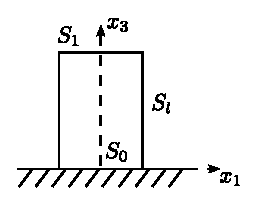
\includegraphics{../images/T1_Ch04-0004}
\end{center}
\end{wrapfigure}
Le bloc est soumis à la seule action de la pesanteur.
En notant $\rho_0 = \rho$, la masse volumique du solide, et $g$, l'accélération de la pesanteur, on a donc
\begin{equation}
    f_1 = f_2 = 0, \quad f_3 = -\rho g
    \label{eq:Ch04-017}
\end{equation}
La surface latérale $S_\ell$ et l'extrémité $S_1(x_3=h)$ sont libres de contraintes
\begin{equation}
    \begin{aligned}
        &\text{sur } S_\ell:\quad && \sigma_{ij} n_j = 0 \\
        &x_3 = h: && \sigma_{13} = \sigma_{23} = \sigma_{33} = 0
    \end{aligned}
    \label{eq:Ch04-018}
\end{equation}
Sur l'extrémité $S_0\ (x_3=0)$, les conditions aux limites dépendent, comme dans le cas précédent, des conditions de contact: dans le cas de non frottement on a
\begin{equation}
    x_3 = 0: \quad u_3 = 0 \quad \sigma_{13} = \sigma_{23} = 0
    \label{eq:Ch04-019}
\end{equation}
et dans le cas de non glissement, on a 
\begin{equation}
    x_3 = 0: \quad u_1 = u_2 = u_3 = 0
    \label{eq:Ch04-020}
\end{equation}

\begin{wrapfigure}{l}{5.5cm}
    \begin{center}
        \includegraphics{../images/T1_Ch04-0005}
    \end{center}
\end{wrapfigure}
Dans le cas du frottement coulombien, on a une expresslon analogue à~\eqref{eq:Ch04-015}.
Toutes ces conditions supposent que le contact entre le bloc et le plan reste maintenu.
Il peut arriver -- figure ci-contre -- qu'une partie du bloc se soulève.
Il s'agit alors d'une liaison unilatérale.
La surface $S_0$ se décompose en deux zones (que l'on ne connaît pas, leur détemination fait partie du problème)
\begin{itemize}
    \item une zone de contact:
        \begin{equation}
            u_3 = 0: \quad \sigma_{33} \leq 0
            \label{eq:Ch04-021}
        \end{equation}
    \item une zone de non contact, libre de contraintes:
        \begin{equation}
            u_3 \geq 0: \quad \sigma_{33} = 0
            \label{eq:Ch04-022}
        \end{equation}
\end{itemize}
On peut regrouper~\eqref{eq:Ch04-021},~\eqref{eq:Ch04-022} en
\begin{equation}
    u_3 \geq 0, \quad \sigma_{33} \leq 0, \quad u_3 \sigma_{33} = 0
    \label{eq:Ch04-023}
\end{equation}
En supposant le contact sans frottement, il faut donc remplacer~\eqref{eq:Ch04-019} par
\begin{equation}
    x_3 = 0:\quad\sigma_{13} = \sigma_{23} = 0, \quad
        u_3 \geq 0, \quad \sigma_{33} \leq 0, \quad u_3 \sigma_{33} = 0
    \label{eq:Ch04-024}
\end{equation}
En toute rigueur, il aurait aussi fallu envisager cette possibilité dans l'exemple précédent, mais elle était peu plausible physiquement.

On pourrait également envisager d'autres types de conditions aux limites sur $S_0$.
\begin{wrapfigure}{l}{3.5cm}
    \begin{center}
        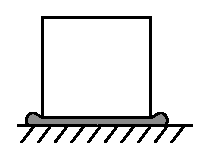
\includegraphics{../images/T1_Ch04-0006}
    \end{center}
\end{wrapfigure}
Par exemple, on peut imaginer de poser le bloc sur le plan par l'intermédiaire d'un ballon de baudruche contenant un gaz à la pression $p$.
Les efforts exercés sur le solide par le ballon se ramènent alors à une pression hydrostatique
\begin{equation}
    x_3 = 0: \quad \sigma_{33} =-p, \sigma_{13} = \sigma_{23} = 0
    \label{eq:Ch04-025}
\end{equation}
On peut déterminer $p$ en remarquant que, d'après les équations d'équilibre, les efforts exercés sur le bloc à travers $S_0$ doivent équilibrer les autres efforts appliqués, en l'occurence, le poids du bloc.
On obtient donc la condition suivante
\begin{equation}
    -\iint_{S_0} \sigma_{33} \ud x_1 \ud x_2 = \rho g S h
    \label{eq:Ch04-026}
\end{equation}
valable quelles que soient les conditions aux limites sur $S_0$.
Avec les conditions~\eqref{eq:Ch04-025}, on en déduit la valeur de $p$
\begin{equation}
    p = \rho g h
    \label{eq:Ch04-027}
\end{equation}
De manière générale, dans un problème réel, l'écriture des conditions aux limites est une étape tout à fait essentielle, car d'une part ces conditions comprennent l'essentiel de la physique du problème, d'autre part elles conditionnent la facilité ---voire la possibilité--- de la résolution du problème mathématique obtenu.
Il faudra souvent faire un compromis entre la précision de la description physique et la facilité de résolution du problème mathématique.

\subsection{Lois de comportement}  \label{ssec:Ch04-1.3}
Pour résoudre un problème de mécanique des solides, il faut donc résoudre un système d'équations aux dérivées partielles.
Pour l'instant, nous avons trois équations scalaires ---les équations du mouvement~\eqref{eq:Ch04-005} ou les équations d'équilibre~\eqref{eq:Ch04-007}, suivant que l'en considère le problème dynamique ou le problème quasi-statique--- pour neuf champs inconnus: trois composantes du déplacement $u_i(x,t)$ et six composantes du tenseur des contraintes $\sigma_{ij}(x,t)$. Il manque donc six équations scalaires.
Ces six équations nous seront fournies par la \emph{loi de comportement} du matériau.
Toutes les équations écrites jusqu'à présent étaient -- dans le cadre d'une schématisation donnée -- -universelles, c'est-à-dire indépendantes du matériau considéré.
Les équations écrites au paragraphe~\ref{ssec:Ch04-1.2} restent les mêmes pour un bloc d'acier, d'aluminium, de matière plastique, de caoutchouc, de bois, de béton, d'argile, de pâte à modeler... sous la seule réserve que les hypothèses fondamentales soient vérifiées (théorie du premier gradient, petites déformations).

De manière générale, la loi de comportement se présente comme une \emph{relation} entre le tenseur des contraintes et le tenseur des déformations.
Cette relation peut être de nature très diverse ---nous en verrons quelques exemples en~\ref{sec:Ch04-2}--- mais elle sera en général de nature \emph{fonctionnelle}.
À quelques cas singuliers près, nous pouvons admettre qu'elle donne le tenseur des contraintes à partir de l'histoire du tenseur des déformations ---c'est-à-dire de la valeur du tenseur des déforrnations à l'instant considéré et à tous les instants antérieurs--- ou bien le tenseur des déformations à partir de l'histoire du tenseur des contraintes.
\begin{equation}
    \tens{\sigma} (t) = \mathop{\tens{\sigma}}_{s=0}^{\infty} \left\{ \tens{\varepsilon} (t-s) \right\}, \quad \tens{\varepsilon} (t) = \mathop{\tens{\varepsilon}}_{s=0}^{\infty} \left\{ \tens{\sigma} (t-s) \right\}
    \label{eq:Ch04-028}
\end{equation}
Cette loi de comportement ne peut être déterminée qu'expérimentalement par un certain nombre d'\emph{essais}.
Les essais les plus faciles à interpréter sont les \emph{essais homogènes} où l'on cherche à réaliser dans une éprouvette, un état de contrainte et de déformation homogène.
L'exemple le plus simple est l'essai de compression simple, qui correspond à l'exemple 2 du paragraphe~\ref{ssec:Ch04-1.2}.
Si l'on cherche un état de contrainte et de déformation homogène
\begin{equation}
    \sigma_{ij} (x,t) = \sigma_{ij}(t), \quad \varepsilon_{ij}(x,t) = \varepsilon_{ij}(t)
    \label{eq:Ch04-029}
\end{equation}
alors la condition aux limites~\eqref{eq:Ch04-008} sur la surface latérale montre que toutes les composantes de $\sigma_{ij}(t)$ sont nulles, sauf $\sigma_{33}$ ---en effet, sur $S_l$ $n_3=0$ tandis que $n_1$ et $n_2$ sont quelconques--- et~\eqref{eq:Ch04-016} donne $\sigma_{33}(t)=-F(t)/S$
\begin{equation}
    \tens{\sigma}(t) = \begin{bmatrix}
        0 & 0 & 0 \\
        0 & 0 & 0 \\
        0 & 0 & -F(t)/S
    \end{bmatrix}
    \label{eq:Ch04-030}
\end{equation}
La loi de conportement~\eqref{eq:Ch04-028} donne alors $\tens{\varepsilon}(t)$ en fonction de $F(t)$.
On obtient alors la forme générale de déplacement par~\eqref{eq:Ch03-062}
\begin{equation}
    \left\{
    \begin{aligned}
        u_1 &= \varepsilon_{11} x_1 + \varepsilon_{12}x_2 + \varepsilon_{13}x_3 + \omega_{2}x_3 - \omega_{3} x_2 +c_1\\
        u_2 &= \varepsilon_{12} x_1 + \varepsilon_{22}x_2 + \varepsilon_{23}x_3 + \omega_{3}x_1 - \omega_{1} x_3 +c_2\\
        u_3 &= \varepsilon_{13} x_1 + \varepsilon_{23}x_2 + \varepsilon_{33}x_3 + \omega_{1}x_2 - \omega_{2} x_1 +c_3
    \end{aligned}
    \right.
    \label{eq:Ch04-031}
\end{equation}
La condition aux limites~\eqref{eq:Ch04-009} en $x_3 =0$ donne alors
\begin{equation*}
    c_3 = 0, \quad \omega_1 = -\varepsilon_{23}, \quad \omega_2 = \varepsilon_{13}
\end{equation*}
La condition aux limites~\eqref{eq:Ch04-009}  en $x_3=h$ est alors vérifiée si
\begin{equation}
    U(t) = -h \varepsilon_{33}(t)
    \label{eq:Ch04-032}
\end{equation}
et il vient
\begin{equation}
    \begin{aligned}
        u_1(x,t) &= \varepsilon_{11}x_1 + (\varepsilon_{12} - \omega_3) x_2 &+ 2\varepsilon_{13}x_3 \\
        u_2(x,t) &= (\varepsilon_{12} + \omega_3) x_1 + \varepsilon_{22}x_2 &+ 2\varepsilon_{23}x_3 \\
        u_3(x,t) &= -U(t) x_3/h
    \end{aligned}
    \label{eq:Ch04-033}
\end{equation}
La solution définie par~\eqref{eq:Ch04-030}, à savoir~\eqref{eq:Ch04-033}, est solution du problème associé au cas sans frottement défini par les conditions aux limites~\eqref{eq:Ch04-011}.
Ainsi, pour réaliser un essai de compression simple, on écrase un lopin en lubrifiant le contact, pour s'approcher au maximum des conditions de non frottement, et en imposant, par exemple, une force $F(t)$ ---essai à force imposée---, la mesure des déplacements donne alors $\tens{\varepsilon}(t)$ et permet donc de déterminer la loi de comportement pour un tenseur $\tens{\sigma}$ de la forme~\eqref{eq:Ch04-030}.

Si le matériau est isotrope ---notion que nous préciserons plus tard--- alors un tenseur $\tens{\sigma}(t)$ de la forme~\eqref{eq:Ch04-030} produit une déformation de la forme
\begin{equation}
    \tens{\epsilon} (t) = 
    \begin{bmatrix}
        \varepsilon_T(t) & 0 & 0 \\
        0 & \varepsilon_T (t) & 0 \\
        0 & 0 & -U(t)/h
    \end{bmatrix}
    \label{eq:Ch04-034}
\end{equation}
La déformation se réduit à un écrasement longitudinal, mesuré par $U(t)$ et une dilatation transversale que l'on mesure facilement à l'aide d'une jauge de déformation.

\subsection{Essais classiques} \label{ssec:Ch04-1.4}
L'essai de compression simple est le prototype des essais homogènes.
L'idée de base est de réaliser un état de contrainte et de déformation homogène qui peut alors être déterminé par des mesures globales d'efforts et de déformation.
Pour les métaux et la plupart des solides, l'essai de base est ``l'essai de traction'', où un barreau cylindrique de longueur $l$ et de section $S$ est soumis à une force longitudinale $F$.
L'état de contrainte et de déformation a la même forme~\eqref{eq:Ch04-030},~\eqref{eq:Ch04-034} que pour l'essai de compression.

\begin{wrapfigure}{l}{3cm}
    \begin{center}
        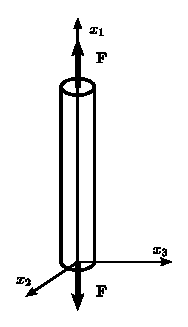
\includegraphics{../images/T1_Ch04-0007}
    \end{center}
\end{wrapfigure}
On mesure 
\begin{itemize}
    \item la force de traction $F(t)$
    \item l'allongement longitudinal $\varepsilon_{l} = \Delta l(t)/l$
    \item l'allongement transfersal $\varepsilon_T(t)$
\end{itemize}
\begin{equation}
    \tens{\sigma} =
    \begin{bmatrix}
        F(t)/S & 0 & 0 \\
        0 & 0 & 0 \\
        0 & 0 & 0
    \end{bmatrix}
    \quad
    \tens{\varepsilon} = 
    \begin{bmatrix}
        \Delta l(t)/l & 0 & 0 \\
        0 & \varepsilon_T(t) & 0 \\
        0 & 0 & \varepsilon_T(t)
    \end{bmatrix}
    \label{eq:Ch04-035}
\end{equation}

Les conditions aux limites~\eqref{eq:Ch04-011} de non frottement sont pratiquement irréalisables, mais on constate expérimentalement que, pourvu que l'éprouvette soit assez longue, alors les résultats de l'essai ne dépendent pratiquement pas de la manière dont est appliquée la force $F$ , c'est-à-dire des conditions aux limites précises sur $S_0$ et $S_\ell$.
C'est le principe de Saint-Venant, sur lequel nous reviendrons au chapitre~\ref{chap:Ch07}.

L'essai de traction est le plus simple à réaliser, mais il ne permet d'obtenir la loi de comportement que pour un tenseur des contraintes de traction ou compression simple.
Cela suffit pour déterminer complètement certaines lois de comportement, mais il est souvent nécessaire de réaliser des états de contrainte plus complexes.
Le choix est alors guidé par la possibilité technologique de réaliser un état de contrainte et déformation le plus homogène possible.
L'essai le plus couramment utilisé pour les métaux est l'essai de ``traction-torsion'' d'un tube mince.
Un tube mince de diamètre $D$, d'épaisseur $e$ et de longueur $l$ est soumis à une force longitudinale $F(t) \vec{e}_3$ et à un couple de torsion $M(t) \vec{e}_3$.

\begin{wrapfigure}[14]{l}{3cm}
    \begin{center}
        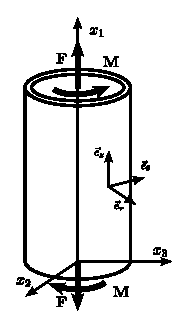
\includegraphics{../images/T1_Ch04-0008}
    \end{center}
\end{wrapfigure}
On mesure
\begin{itemize}
    \item l'allongement longitudinal $\Delta l(t)/l$
    \item l'allongement transversal $\varepsilon_T(t)$
    \item la rotation relative $\Delta \theta(t)$ des deux sections extrémités.
\end{itemize}
Pourvu que le le tube soit suffisament mince, l'état de contrainte et de déformation est donné dans le repère local $\left(\vec{e}_r, \vec{e}_{\theta}, \vec{e}_z  \right)$ associé aux coordonnées cylindrique par
\begin{equation}
    \tens{\sigma} =
    \begin{bmatrix}
        0 & 0 & 0 \\
        0 & 0 & 2M/\pi D^2 e \\
        0 & 2M/\pi D^2 e & F/\pi D e
    \end{bmatrix}
    \quad
    \tens{\varepsilon} = 
    \begin{bmatrix}
        \varepsilon_T & 0 & 0 \\
        0 & \varepsilon_T & D \Delta \theta / 4 l \\
        0 & D \Delta \theta / 4 l & \Delta l/l
    \end{bmatrix}
    \label{eq:Ch04-036}
\end{equation}
superposition d'une traction simple et d'un cisaillement simple.

Ce type d'essai convient pour des matériaux suffisamment consistants.
En mécanique des sols, où l'on a affaire à des matériaux peu ou pas cohérents, on utilise classiquement deux types d'essais.

\begin{wrapfigure}[8]{l}{3cm}
    \begin{center}
        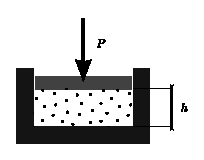
\includegraphics{../images/T1_Ch04-0009}
    \end{center}
\end{wrapfigure}
Dans l'essai oediométrique, on comprime le matériau dans un moule rigide.
On réalise ainsi un état de contrainte et de déformation de la forme
\begin{equation}
    \tens{\varepsilon} =
    \begin{bmatrix}
        \Delta h/h & 0 & 0 \\
        0 & 0 & 0 \\
        0 & 0 & 0
    \end{bmatrix}
    \quad
    \tens{\sigma} = 
    \begin{bmatrix}
        P/S & 0 & 0 \\
        0 & \sigma_T & 0 \\
        0 & 0 & \sigma_T
    \end{bmatrix}
    \label{eq:Ch04-037}
\end{equation}

\begin{wrapfigure}[10]{l}{3cm}
    \begin{center}
        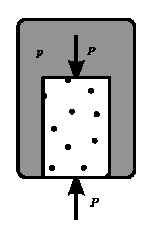
\includegraphics{../images/T1_Ch04-0010}
    \end{center}
\end{wrapfigure}
Dans l'essai ``triaxial'', on place une éprouvette dans une cellule triaxiale que l'on soumet à une pression $p$ et on superpose une force longitudinale $P$.
On réalise ainsi un état de contrainte et de déformation de révolution (paragraphe~\ref{ssec:Ch02-1.3})
\begin{equation}
    \tens{\varepsilon} =
    \begin{bmatrix}
        \varepsilon_L & 0 & 0 \\
        0 & \varepsilon_T & 0 \\
        0 & 0 & \varepsilon _T
    \end{bmatrix}
    \quad
    \tens{\sigma} = 
    \begin{bmatrix}
        p + P/S & 0 & 0 \\
        0 & p & 0 \\
        0 & 0 & p
    \end{bmatrix}
    \label{eq:Ch04-038}
\end{equation}

Tous ces essais homogènes présentent l'avantage de pouvoir s'interpréter directement en termes de loi de comportement.
Mis à part l'essai de traction, ils présentent cependant l'inconvénient d'être assez fins, nécessitant de grandes précautions pour obtenir des résultats significatifs.
Dans la pratique courante, on utilise souvent des essais non homogènes, souvent issus de la tradition (essai pénétrornétrique en Mécanique des Sols, essai de dureté ou de résilience pour les métaux) qui permettent d'obtenir simplement des caractéristiques globales du comportement.
Malheureusement, ces essais ne fournissent sur les lois de comportement que des informations qualitatives, que l'on ne peut pas utiliser directement.

\section{Comportement des solides} \label{sec:Ch04-2}
\subsection{Diversité des comportements} \label{ssec:Ch04-2.1}
Le but de ce paragraphe est double: d'une part nous allons décrire quelques uns des types de comportement que l'on peut rencontrer; d'autre part nous allons introduire la terminologie utilisée pour caractériser ces comportements.

Pour les métaux à température ambiante, le comportement est convenablement décrit par la courbe de traction, résultat de l'essai de traction.
On fait croître la force $F$ et on mesure l'allongement longitudinal $\varepsilon_L$.
\begin{multicols}{2}
    \begin{center}
        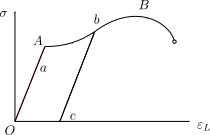
\includegraphics{../images/T1_Ch04-0011}

        Acier doux
    \end{center}
    \columnbreak
    \begin{center}
        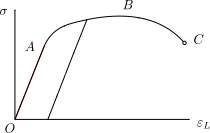
\includegraphics{../images/T1_Ch04-0012}

        Acier durs, métaux non ferreux
    \end{center}
\end{multicols}
La courbe se divise en trois régions.
La région $OA$ correspond à un comportement élastique linéaire, dont les deux caractéristiques essentielles sont:
\begin{itemize}
    \item réversibilité: si, arrivé au point $a$ on diminue la contrainte, on redescend suivant la même courbe;
    \item linéarité: la contrainte est proportionnelle à la déformation. 
\end{itemize}
Cette région correspond à la déformation réversible du réseau cristallin. 

A partir du seuil $A$, on entre dans la zone $AB$ de comportement plastique, essentiellement caractérisé par son irréversibilité: si, arrivé en $b$ on décharge, alors on redescend, non pas le long de la courbe de charge $b\ A$, mais sur une droite $bc$ parallèle à $OA$.
En fait le comportement est alors à nouveau élastique tant que l'on ne redépasse pas le nouveau seuil $b$.
En particulier, on constate que la déformation plastique entre $A$ et $b$ a eu comme effet d'élargir la région élastique.
C'est le phénomène d'écrouïssage.

Le point $B$ correspond à l'apparition de la striction -- instabilité géométrique qui conduit à la localisation de la déformation.
La contrainte $\sigma$ diminue alors jusqu'à rupture.
En fait, il s'agit de la contrainte apparente, c'est-à-dire ramenée à la surface initiale, la contrainte vraie, c'est-à-dire ramenée à la surface réelle de la striction, elle, continue à augmenter.
De toute façon, la déformation n'est plus homogène, et cette portion de courbe ne décrit pas directement le comportement.
De plus, l'hypothèse des petites déformations n'est plus vérifiée.
\begin{multicols}{2}
    \begin{center}
        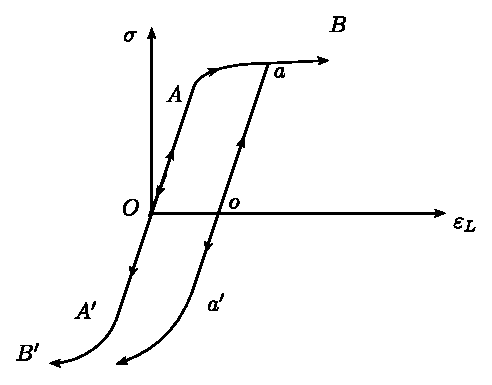
\includegraphics{../images/T1_Ch04-0013}
    \end{center}
    \columnbreak
    \begin{center}
        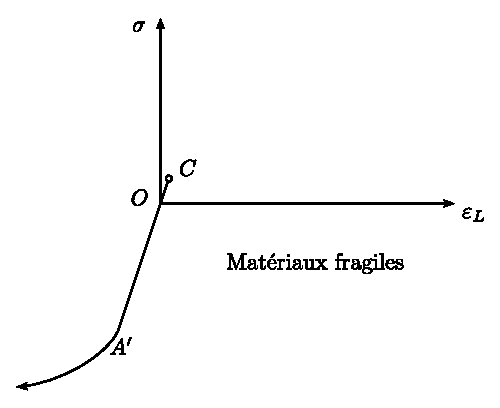
\includegraphics{../images/T1_Ch04-0014}
    \end{center}
\end{multicols}
En compression simple, on obtient en général un comportement symétrique $OA'B'$ (mais sans striction).
Pour certains matériaux fragiles (béton, fonte, roches, etc.), cependant, on obtient en compression simple un comportement ductile, comme celui que nous avons décrit, et en traction simple, un comportement fragile conduisant à rupture très rapide.
Pour les métaux, on observe souvent l'effet Bauschinger: après une précharge $OAa$ en traction, l'écrouissage qui se traduit par une augmentation du seuil en traction, entraîne également une diminution du seuil en compression, alors qu'au départ les deux étaient approximativement égaux.

La courbe de traction permet également de décrire le comportement d'autres matériaux, comme le caoutchouc, (comportement élastique non linéaire en première approximation) ou les sols -- on représente alors le résultat d'un essai «~triaxial~» à $p$ fixé -- qui présentent un comportement de type élasta-plastique avec une région élastique très réduite et avec ou sans pic suivant que le matériau est initialement plus ou moins tassé.
\begin{multicols}{2}
    \begin{center}
        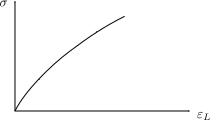
\includegraphics{../images/T1_Ch04-0015}

        caoutchouc
    \end{center}
    \columnbreak
    \begin{center}
        \includegraphics{../images/T1_Ch04-0016}

        sols
    \end{center}
\end{multicols}

Pour des matériaux comme les matières plastiques ou les métaux à haute température, la courbe de traction perd toute signification, car elle dépend de manière cruciale de la vitesse de déformation.
On caractérise alors le comportement par des essais de fluage et de relaxation.
Pour l'essai de fluage, toujours en traction ou compression simple, on impose une contrainte constante et on observe la déformation en fonction du temps: l'application de la contrainte s'accompagne d'une déformation instantanée, puis la déformation se poursuit, puis se stabilise, soit vers une constante, soit vers un état de fluage stationnaire à vitesse de déformation constante.
\begin{multicols}{2}
    \begin{center}
        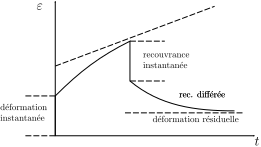
\includegraphics{../images/T1_Ch04-0017}

        Matériau de type fluide
    \end{center}
    \columnbreak
    \begin{center}
        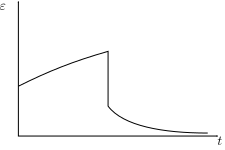
\includegraphics{../images/T1_Ch04-0018}

        Solide
    \end{center}
\end{multicols}
Si à un l'instant $t_0$ on relache la contrainte, alors la déformation de décompose en trois port parties:
\begin{itemize}
    \item une déformation instantanée (recouvrance instantanée),
    \item une déformation obtenue progressivement (recouvrance différée),
    \item une déformation résiduelle qui subsiste,
\end{itemize}
cette dernière pouvant disparaître pour un matériau de type solide.

L'essai de relaxation consiste à appliquer une déformation constante, et à observer la contrainte nécessaire
\begin{multicols}{2}
    \begin{center}
        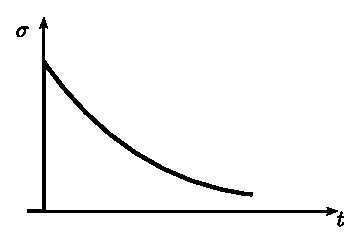
\includegraphics{../images/T1_Ch04-0019}

        Fluide
    \end{center}
    \columnbreak
    \begin{center}
        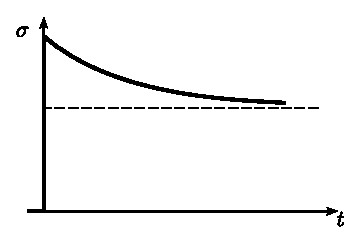
\includegraphics{../images/T1_Ch04-0020}

        Solide
    \end{center}
\end{multicols}

Si l'on pousse plus loin l'essai de fluage, on voit apparaître après le fluage primaire (régime transitoire) et le fluage secondaire (régime stabilisé) une zone de fluage tertiaire qui correspond au phénomène «~d'endommagement~» (détérioration du matériau qui conduit à la rupture).
\begin{multicols}{2}
    \begin{center}
        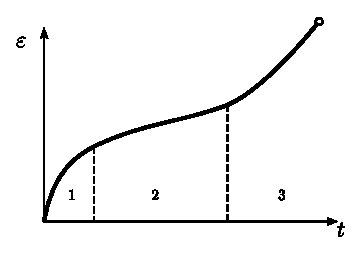
\includegraphics{../images/T1_Ch04-0021}
    \end{center}
    \columnbreak
    \begin{enumerate}
        \item fluage primaire
        \item fluage secondaire
        \item fluage tertiaire
    \end{enumerate}
\end{multicols}

Ce type de comportement dépendant du temps est appelé «~viscoplastique~»  ou «~viscoélastique~», selon qu'il existe ou non un seuil en dessous duquel le comportement peut être considéré comme élastique.
En première approximation, les matières plastiques ont un comportement viscoélastique, et les métaux à haute température un comportement viscoplastique.

\subsection{Modèles rhéologiques} \label{ssec:Ch04-2.2}
Il est important de savoir construire des modèles mathématiques de comportement décrivant, au moins qualitativement, les différents types de comportement que nous venons de présenter.
Les modèles rhéologiques forment une classe déjà très vaste de tels modèles.
Ils s'obtiennent par combinaison de 3 modèles élémentaires
\begin{itemize}
    \item le ressort, modèle de comportement élastique
        \begin{multicols}{2}
            \begin{equation}
                \sigma = E \varepsilon
                \label{eq:Ch04-039}
            \end{equation}
            \columnbreak
            \begin{center}
                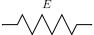
\includegraphics{../images/T1_Ch04-0022}
            \end{center}
        \end{multicols}
    \item le patin, modèle de comportement plastique
        \begin{multicols}{2}
            \begin{equation}
                \begin{cases}
                    \dot\varepsilon = 0 & \text{ si } |\sigma|<\sigma_0 \\
                    \dot\varepsilon > 0 & \text{ si } |\sigma|=\sigma_0 \\
                    \dot\varepsilon < 0 & \text{ si } |\sigma|=-\sigma_0
                \end{cases}
                \label{eq:Ch04-040}
            \end{equation}
            \columnbreak
            \begin{center}
                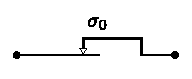
\includegraphics{../images/T1_Ch04-0023}
            \end{center}
        \end{multicols}
    \item l'amortisseur, modèle de comportement visqueux
        \begin{multicols}{2}
            \begin{equation}
                \sigma = \eta \dot \varepsilon
                \label{eq:Ch04-041}
            \end{equation}
            \columnbreak
            \begin{center}
                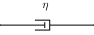
\includegraphics{../images/T1_Ch04-0024}
            \end{center}
        \end{multicols}
\end{itemize}
Les modèles rhéologiques s'obtiennent par montage en parallèle (les contraintes s'additionnent, les deformations sont les mêmes) ou en série (les déformations s'additionnent, les contraintes sont les mêmes).

Le comportement viscoélastique peut être représenté par une combinaison de ressorts et d'amortisseurs. 
\begin{itemize}
    \item Par montage en série d'un ressort et d'un amortisseur, on obtient le modèle de Maxwell:
        \begin{multicols}{2}
            \begin{equation}
                \left\{
                \begin{aligned}
                    \sigma &= E \varepsilon_1 = \eta \dot{\varepsilon}_2 \\
                    \varepsilon &= \varepsilon_1 + \varepsilon_2
                \end{aligned}
                \right.
                \label{eq:Ch04-042}
            \end{equation}
            ou en éliminant $\varepsilon_1$ et $\varepsilon_2$
            \begin{equation}
                \dot \varepsilon = \frac{\dot \sigma}{E} + \frac{\sigma}{\eta}
                \label{eq:Ch04-043}
            \end{equation}
            \columnbreak
            \begin{center}
                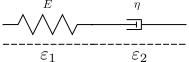
\includegraphics{../images/T1_Ch04-0025}
            \end{center}
        \end{multicols}
        qui est la loi de comportement sous forme différentielle.
        Conformément à~\eqref{eq:Ch04-028}, on voit que, connaissant l'histoire de $\sigma$ (ou de $\varepsilon$), on peut en déduire la valeur à l'instant $t$ de $\varepsilon$ (ou de $\sigma$ par intégration de l'équation différentielle~\eqref{eq:Ch04-043}.
    \item Par montage en parallèle d'un ressort et d'un amortisseur, on obtient le modèle de Kelvin-Voigt
        \begin{multicols}{2}
            \begin{equation}
                \left\{
                \begin{aligned}
                    \sigma &= E \varepsilon_1 = \eta_2 \dot{\varepsilon}_2 = E_3 \varepsilon_3 + \eta_3 \dot \varepsilon_3 \\
                    \varepsilon &= \varepsilon_1 + \varepsilon_2 + \varepsilon_3
                \end{aligned}
                \right.
                \label{eq:Ch04-045}
            \end{equation}
            \columnbreak
            \begin{center}
                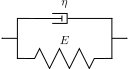
\includegraphics{../images/T1_Ch04-0026}
            \end{center}
        \end{multicols}
    \item Par montage en série-d'un modèle de-Maxwell et d'un modèle de Kelvin-Voigt, on obtient le modèle de Burgers
        \begin{multicols}{2}
            \begin{equation}
                \sigma = E \varepsilon + \eta \dot \varepsilon
                \label{eq:Ch04-044}
            \end{equation}
            \columnbreak
            \begin{center}
                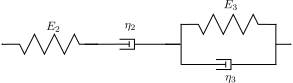
\includegraphics[scale=0.8]{../images/T1_Ch04-0027}
            \end{center}
        \end{multicols}
        En éliminant $\varepsilon_1$, $\varepsilon_2$ et $\varepsilon_3$, il vient
        \begin{equation}
            \ddot \varepsilon + \frac{E_3}{\eta_3} \dot{\varepsilon} = \frac{1}{E_1} \ddot{\sigma} + \left( \frac{E_3}{\eta_3E_1} + \frac{1}{\eta_2} + \frac{1}{\eta_3} \right)\dot{\sigma} + \frac{E_3}{\eta_2\eta_3} \sigma
            \label{eq:Ch04-046}
        \end{equation}
        forme différentielle de la loi de comportement.
        En particulier, on obtient en fluage une courbe qui représente qualitativement le comportement de certaines matières plastiques.
\end{itemize}
Et ainsi de suite.

Les comportements élasto-plastiques s'obtiennent par combinaison de ressorts et de patins.
\begin{itemize}
    \item Par montage en série d'un ressort et d'un patin, on obtient un modèle élasto-plastique sans écrouissage
        \begin{center}
            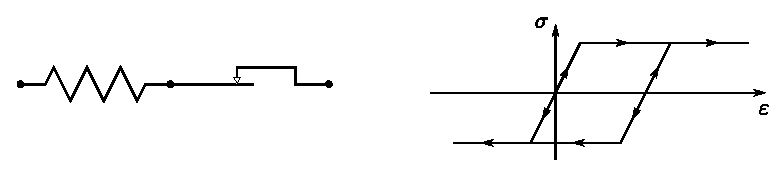
\includegraphics{../images/T1_Ch04-0028}
        \end{center}
    \item On obtient un modèle avec écrouissage linéaire montage suivant
        \begin{center}
            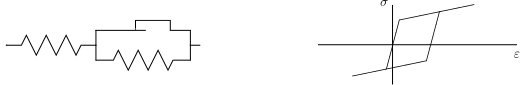
\includegraphics{../images/T1_Ch04-0029}
        \end{center}
\end{itemize}

\begin{wrapfigure}{l}{6cm}
    \begin{center}
        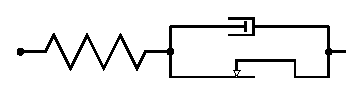
\includegraphics{../images/T1_Ch04-0030}
    \end{center}
\end{wrapfigure}
Enfin, on peut obtenir des comportements viscoplastiques par des combinaisons des trois éléments de base.
Par exemple le modèle de Bingham permet de décrire le comportement du goudron et de certaines pâtes.

De manière générale, le choix d'un modèle représentant le comportement d'un matériau réel est un problème difficile.
Le comportement des matériaux réels est complexe, et nous n'en avons présenté qu'une esquisse très  incomplète.
Même pour des matériaux aussi courants que l'acier, de nombreux aspects du comportement restent mal connus, et il est impossible de  construire un modèle représentant le comportement d'un matérjau donné en toutes circonstances.
Dans chaque problème, il convient de choisir le modèle le plus simple conduisant à des résultats satisfaisants pour l'utilisation qu'on veut en faire.
Dans certains cas, en particulier si l'on recherche une grande fiabilité, il conviendra de faire le calcul avec une loi de comportement très sophistiquée, prenant en compte tous les risques de ruine possibles, ces calculs étant rendus possibles par les développements de l'informatique.
Dans d'autres cas, par contre, on pourra se satisfaire d'approximations plus grossières du comportement, et c'est la raison d'être des modèles élémentaires qui feront l'objet de la suite de ce cours.

